% =====================================================================
%  Section 7 - Results (author's edits in 7.1-7.5)
%  Every number below is from Results/stats/*, NoiseStudy/report.txt
%  and the released results.json / results_fixedbase.json.
% =====================================================================
\section{Results}
\label{sec:results}

All errors in this section are re-evaluated errors (Sect.~\ref{sec:reeval}), given as medians over the 30 seeds, and lower is better. Table~\ref{tab:main} gives every method at every mutation strength for both stages.

\begin{table}[!htb]
\centering
\caption{Median re-evaluated error over 30 seeds (lower is better). SS = steady-state, EL = elitist generational, GEN = generational. Bold: within one noise floor of the best value in its column (0.0298 base, 0.088 free, Sect.~\ref{sec:stats}).}
\label{tab:main}
\setlength{\tabcolsep}{3.5pt}
\footnotesize
\begin{tabular}{@{}lcccccccc@{}}
\toprule
 & \multicolumn{4}{c}{Base stage, $m =$} & \multicolumn{4}{c}{Free stage, $m =$} \\
\cmidrule(lr){2-5}\cmidrule(l){6-9}
Method & 1 & 3 & 5 & 10 & 1 & 3 & 5 & 10 \\
\midrule
SS + Tournament & \textbf{0.076} & \textbf{0.114} & \textbf{0.090} & \textbf{0.139} & 2.032 & \textbf{1.303} & 1.347 & 1.797 \\
SS + Roulette & 0.163 & 0.137 & 0.150 & 0.206 & 2.008 & 1.356 & 1.718 & 1.766 \\
SS + SUS & 0.140 & 0.153 & \textbf{0.091} & 0.169 & 2.072 & \textbf{1.262} & 1.489 & 1.593 \\
EL + Tournament & 0.176 & 0.119 & \textbf{0.100} & 0.210 & 2.021 & 1.423 & \textbf{1.174} & 1.601 \\
EL + Roulette & 0.155 & \textbf{0.086} & 0.132 & 0.269 & 1.940 & 1.363 & 1.474 & \textbf{1.574} \\
EL + SUS & 0.135 & 0.151 & 0.148 & 0.221 & \textbf{1.828} & 1.479 & 1.431 & 1.730 \\
GEN + Tournament & 0.169 & 0.158 & 0.209 & 0.522 & 2.010 & 1.706 & 1.870 & 1.990 \\
GEN + Roulette & 0.252 & 0.349 & 0.445 & 1.555 & 2.069 & 1.907 & 2.001 & 2.059 \\
GEN + SUS & 0.173 & 0.234 & 0.333 & 0.830 & \textbf{1.885} & 1.729 & 1.900 & 1.952 \\
\midrule
Hill climbing & 0.160 & 0.118 & \textbf{0.084} & \textbf{0.128} & 1.988 & 1.780 & 1.559 & \textbf{1.527} \\
Simulated annealing & 0.192 & 0.130 & \textbf{0.075} & \textbf{0.155} & 1.926 & 1.532 & 1.277 & \textbf{1.494} \\
Random search & 37.5 & 37.5 & 37.5 & 37.5 & 62.8 & 62.8 & 62.8 & 62.8 \\
\bottomrule
\end{tabular}
\end{table}

\subsection{Automatic Tuning Works}
\label{sec:res-works}

In the base stage, the best of the 10 random starting reel sets has a median error of about 97. With 1000 evaluations, every method except random search brings this down to between 0.075 and 0.25 at its best mutation strength, and most of them to around 0.1 (Table~\ref{tab:main}). An error of 0.1 means, for example, a base RTP that is 1\% off its target with the other two stats exact. Random search, with the same budget, stays at 37.5 and loses to every GA configuration on 30 of 30 seeds at every mutation strength ($p_{\mathrm{Holm}} < 0.001$, $A_{12} = 1.00$), so the result comes from the search itself and not from luck.

\subsection{Replacement, Selection and Mutation}
\label{sec:res-ga}

\paragraph{Replacement decides the result.} Generational replacement is the worst scheme, and the gap grows with mutation strength. Against steady-state, its median error is 0.185 vs 0.145 at $m = 1$, 0.214 vs 0.144 at $m = 3$, 0.333 vs 0.144 at $m = 5$ and 0.707 vs 0.162 at $m = 10$, where it loses on 30 of 30 seeds ($A_{12} = 1.00$, $p_{\mathrm{Holm}} < 0.001$). Elitist replacement beats generational in the same way from $m = 3$ upwards. The result at $m = 1$ is the weakest one ($p_{\mathrm{Holm}} = 0.044$, Friedman $p = 0.107$). Steady-state and elitist replacement are tied at $m = 1$, 3 and 5. Only at $m = 10$ is steady-state better (0.162 vs 0.224, $p_{\mathrm{Holm}} = 0.007$, $A_{12} = 0.72$).

\paragraph{Selection matters only without elitism.} Inside steady-state and inside elitist replacement, no pair of selection methods differs significantly at any mutation strength. Inside generational replacement, selection does matter: Tournament beats Roulette at every $m$, SUS beats Roulette at every $m$, and Tournament beats SUS from $m = 3$ upwards.

\paragraph{Gentle mutation is better.} Changing 10 of the 250 positions is significantly worse than a smaller $m$ for 9 of the 11 methods. The damage is largest for generational replacement: Generational + Roulette goes from 0.252 at $m = 1$ to 1.555 at $m = 10$.
\subsection{GA versus Local Search}
\label{sec:res-baselines}

In the base stage, no GA configuration is significantly better than hill climbing or simulated annealing at any mutation strength. With each method at its own best mutation strength, the best GA (SS + Tournament, $m = 1$) and simulated annealing ($m = 5$) reach 0.076 and 0.075, simulated annealing is lower on 15 of the 30 seeds, $A_{12} = 0.53$ and $p_{\mathrm{Holm}} = 1.0$, i.e.\ a draw.
In the other direction, the baselines are significantly better than every generational configuration at $m = 5$ and 10, so in the base stage the best a well-configured GA can do is a draw, and a badly configured GA loses to local search.

\subsection{Free Game and Fixed-Base Check}
\label{sec:res-free}

The free stage has a higher error, with best medians of 1.17 to 1.30 against about 0.1 in the base stage, because the free-game targets pull against each other (Fig.~\ref{fig:tradeoff}). The ranking of methods is similar: steady-state and elitist replacement are at the top, level with simulated annealing, and generational replacement is significantly worse than both at $m = 3$, 5 and 10 ($A_{12}$ from 0.80 to 0.94). Three things differ. First, $m = 1$ is now the worst mutation strength for 10 of the 11 methods. Second, elitist replacement beats steady-state at $m = 1$ and 5 ($p_{\mathrm{Holm}} = 0.030$ and 0.009, $A_{12} = 0.65$). Third, all six steady-state and elitist configurations beat hill climbing at $m = 3$, e.g.\ SS + SUS with 1.262 vs 1.780 on 27 of 30 seeds ($A_{12} = 0.83$, $p_{\mathrm{Holm}} < 0.001$), whereas no GA configuration beats simulated annealing at any $m$. Selection again matters mainly inside generational replacement (one exception: EL + SUS beat EL + Tournament at $m = 1$, $p_{\mathrm{Holm}} = 0.034$).

With the fixed base reels, the median error over the 990 paired runs barely moves (1.661 vs 1.649, Wilcoxon $p = 0.77$), the ranking is kept (Spearman $\rho = 0.84$), and the same findings hold, except that only three configurations beat hill climbing at $m = 3$ (SS + SUS, SS + Tournament and EL + SUS). So the free-stage findings do not come from the base reels.

\begin{figure}[t]
\centering
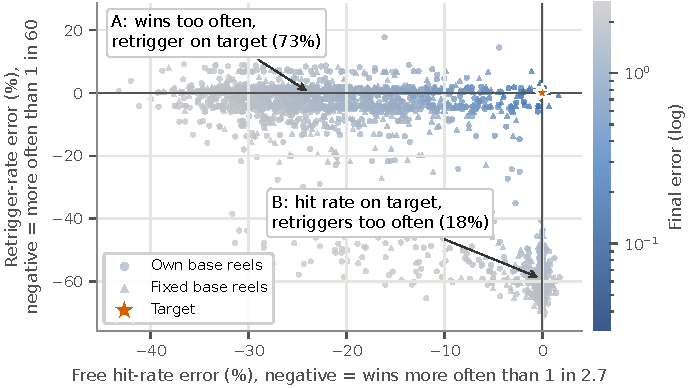
\includegraphics[width=\textwidth]{figures/free_tradeoff.pdf}
\caption{Free stage: error in free hit rate against error in retrigger rate (in \%) for the 2310 final free reel sets, with each method's own base reels (circles) and with the fixed base reels (triangles), random search excluded. Colour shows the final error; the target is the star at (0, 0). Most reel sets fall into two groups: A hits the retrigger target but wins too often, and B hits the hit-rate target but retriggers too often.}
\label{fig:tradeoff}
\end{figure}

Of the 2310 final free reel sets, 73\% hit the retrigger target but win too often, 18\% hit the free hit-rate target but retrigger far too often, and only 16 (0.7\%) reach an error of 0.25 or less. Every retrigger adds 10 spins, so more retriggers mean longer rounds and more free RTP. With this game's symbols and rules the free-game targets appear to conflict, and every method has to trade one against the other.

\subsection{Noise Study}
\label{sec:noisestudy}

Re-simulating the best reel sets 30 times each with $10^7$ spins, the standard deviation of the error is about 0.013 in the base stage and 0.035 in the free stage (medians over reel sets), almost the same for every method except random search, since it comes from the simulator and not from the optimiser. For a given method and $m$, the spread of final errors between seeds (interquartile range) is a median 4.3 times the noise floor in the base stage and 5.6 times in the free stage, so the outcome of a run is decided by the search, not by measurement error. The in-run best is optimistic: in the base stage the re-evaluated median is higher than the in-run median in 36 of 44 method--mutation combinations (median ratio 1.04), and in one case by a factor of 1.63 (SS + Tournament at $m = 1$: 0.047 during the run, 0.076 on re-evaluation); in the free stage the ratios lie between 0.98 and 1.07.
Finally, every significant difference reported above is also larger than the noise floor: all 75 in the base stage, 67 in the free stage and 27 in the fixed-base check. However, noise does limit the order among the best GA configurations and the baselines, as their differences are within the noise floor in the base stage, and that is why they are reported as tied rather than ranked.
